%%%%%%%%%%%%%%%%%%%%%%%%%%%%%%%%%%%%%%%%%
% Short Sectioned Assignment
% LaTeX Template
% Version 1.0 (5/5/12)
%
% This template has been downloaded from:
% http://www.LaTeXTemplates.com
%
% Original author:
% Frits Wenneker (http://www.howtotex.com)
%
% License:
% CC BY-NC-SA 3.0 (http://creativecommons.org/licenses/by-nc-sa/3.0/)
%
%%%%%%%%%%%%%%%%%%%%%%%%%%%%%%%%%%%%%%%%%

%----------------------------------------------------------------------------------------
%	PACKAGES AND OTHER DOCUMENT CONFIGURATIONS
%----------------------------------------------------------------------------------------

%% \documentclass[paper=a4, fontsize=11pt]{scrartcl} % A4 paper and 11pt font size
\documentclass[paper=letter, fontsize=12pt]{scrartcl} % Letter paper and 12pt font size

\usepackage[utf8]{inputenc}
\usepackage[T1]{fontenc} % Use 8-bit encoding that has 256 glyphs
\usepackage{fourier} % Use the Adobe Utopia font for the document - comment this line to return to the LaTeX default
\usepackage[spanish]{babel} % English language/hyphenation
\usepackage{amsmath,amsfonts,amsthm} % Math packages
\usepackage{listings}
\usepackage{xcolor}

\lstset{literate=
  {á}{{\'a}}1 {é}{{\'e}}1 {í}{{\'i}}1 {ó}{{\'o}}1 {ú}{{\'u}}1
  {Á}{{\'A}}1 {ñ}{{\~n}}1 {É}{{\'E}}1 {Í}{{\'I}}1 {Ó}{{\'O}}1
  {Ú}{{\'U}}1 {π}{{pi}}1,
  belowcaptionskip=1\baselineskip,
  breaklines=true,
  frame=L,
  xleftmargin=\parindent,
  language=R,
  showstringspaces=false,
  basicstyle=\footnotesize\ttfamily,
  keywordstyle=\bfseries\color{green!40!black},
  commentstyle=\itshape\color{purple!40!black},
  identifierstyle=\color{blue},
  stringstyle=\color{orange},
}

\usepackage{indentfirst}
\usepackage{lipsum} % Used for inserting dummy 'Lorem ipsum' text into the template
\usepackage{sectsty} % Allows customizing section commands
\allsectionsfont{\raggedright \textit\normalfont\scshape\emph} % Make all sections centered, the default font and small caps

\usepackage{fancyhdr} % Custom headers and footers
\pagestyle{fancyplain} % Makes all pages in the document conform to the custom headers and footers
\fancyhead{} % No page header - if you want one, create it in the same way as the footers below
\fancyfoot[L]{} % Empty left footer
\fancyfoot[C]{} % Empty center footer
\fancyfoot[R]{\thepage} % Page numbering for right footer
\renewcommand{\headrulewidth}{0pt} % Remove header underlines
\renewcommand{\footrulewidth}{0pt} % Remove footer underlines
\setlength{\headheight}{13.6pt} % Customize the height of the header

\numberwithin{equation}{section} % Number equations within sections (i.e. 1.1, 1.2, 2.1, 2.2 instead of 1, 2, 3, 4)
\numberwithin{figure}{section} % Number figures within sections (i.e. 1.1, 1.2, 2.1, 2.2 instead of 1, 2, 3, 4)
\numberwithin{table}{section} % Number tables within sections (i.e. 1.1, 1.2, 2.1, 2.2 instead of 1, 2, 3, 4)
\usepackage{graphicx}
\graphicspath{ {./images/} }

\setlength\parindent{0pt} % Removes all indentation from paragraphs - comment this line for an assignment with lots of text


%----------------------------------------------------------------------------------------
%	TITLE SECTION
%----------------------------------------------------------------------------------------

\newcommand{\horrule}[1]{\rule{\linewidth}{#1}} % Create horizontal rule command with 1 argument of height

\title{
  \vspace*{\fill}
  \begin{center}
    \normalfont \normalsize
    \textsc{Universidad Nacional Autónoma de México\\Facultad de Ciencias} \\ [25pt]
    \horrule{0.5pt} \\[0.4cm] % Thin top horizontal rule
    \huge \textbf{Tarea Examen 1} \\ % The assignment title
    \horrule{2pt} \\[0.5cm] % Thick bottom horizontal rule
    \large \textit{Procesos Estocásticos} \\
  \end{center}
}

\author{Arroyo Jamaica Juan Manuel\\González Velasco María Fernanda\\
  Leyva Pichardo Jesús Francisco\\Luna Soto Ileana\\Orozco Camacho Albert Manuel}

\date{\normalsize\today} % Today's date or a custom date
\begin{document}

\begin{titlepage}
  \maketitle
  \thispagestyle{empty}
  \vspace*{\fill}
\end{titlepage}

\section{Consideraciones generales con respecto a las simulaciones y sus códigos}

\begin{itemize}
\item En cada script presentado a continuación, se omitieron las funciones \textit{print} y\
  \textit{plot}. Esto con el fin de hacer el código más corto (ya que esto se va a imprimir) y\
  legible. El código enviado por correo es el mismo del presentado aquí pero con los detalles\
  omitidos.
\item Por lo anterior, se recomienda \textbf{NO} correr directamente el código impreso en este\
  documento, sino utilizar el que fue enviado por correo.
\item Algunas parámetros de las simulaciones se determinan aleatoriamente. Es aconsejable correr\
  más de una vez todos los scripts para poder apreciar el comportamiento de las funciones bajo\
  distintos parámetros.
\item Cada gráfico impreso fue resultado de una ejecución del código en cuestión. Las formas de los\
  gráficos pueden variar por ejecución.
\item Se recomienda \textbf{altamente} no ejecutar un script sin cerrar las ventanas con gráficos\
  que aparecieron en alguna ejecución anterior.
\item Antes de ejecutar cualquier script, se recomienda cerciorarse de que todos los scripts estén\
  guardados en una misma carpeta.
\end{itemize}

\section{Funciones generales usadas para las simulaciones}

En el siguiente script se muestran varias funciones implementadas de uso común para varias\
de las simulaciones pedidas a lo largo de la tarea examen.

\lstinputlisting[language=R]{../funciones_generales.R}

\section{Ejercicio 1}

\subsection{Código}

\lstinputlisting[language=R]{../ejercicio1.R}

\subsection{Gráficos}

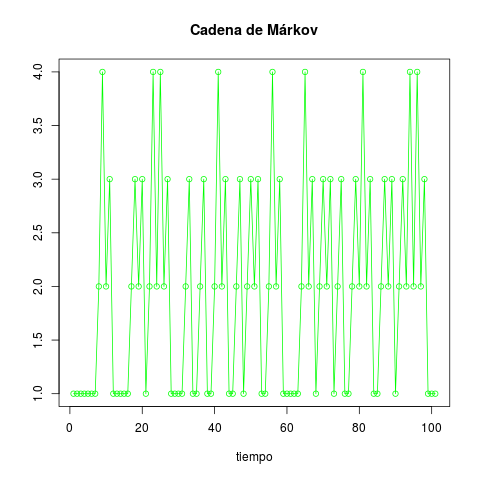
\includegraphics[scale=0.5]{ej1_1.png}
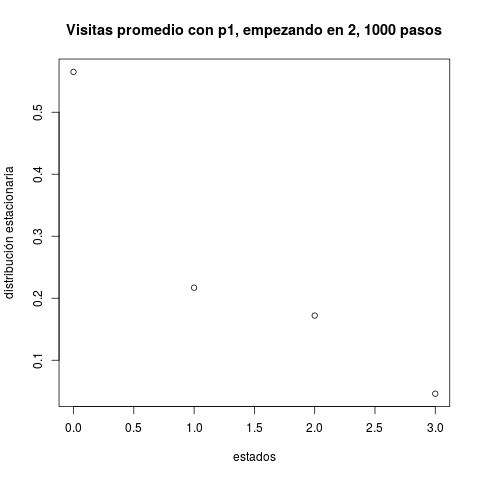
\includegraphics[scale=0.5]{ej1_2.png} 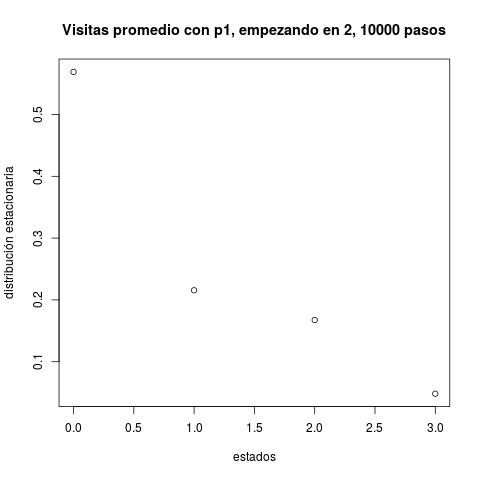
\includegraphics[scale=0.5]{ej1_3.png}
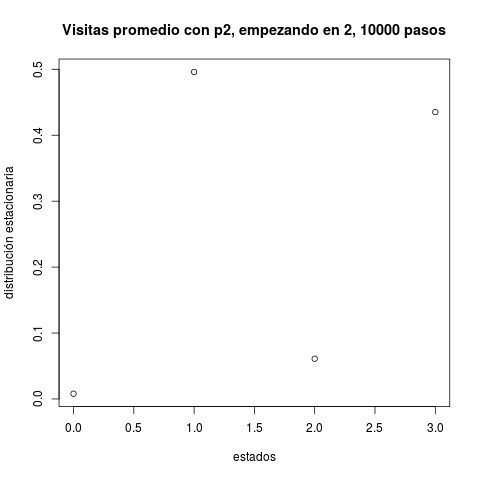
\includegraphics[scale=0.5]{ej1_4.png} 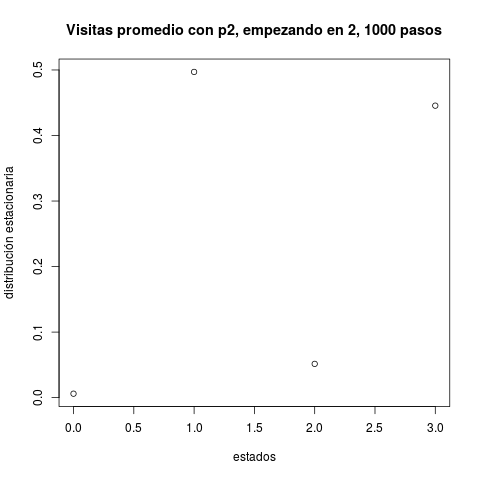
\includegraphics[scale=0.5]{ej1_5.png}

\section{Ejercicio 3}

\subsection{Código}

La función que simula la cadena de Márkov en cuestión usa varias funciones auxiliares.\
Esto está motivado a que se debe guardar el tiempo de vida de cada partícula que ingresa\
al cuerpo en cada tiempo. Entonces, se utiliza un vector cuyo tamaño es el número de partículas\
en un tiempo $n$ y en cada entrada se guarda el tiempo de vida de cada partícula.\par
En cada iteración, la función actualiza dicho vector, \textit{elimina las partículas muertas}\
y obtiene las partículas que siguen vivas. Es decir, en cada iteración se calculan las partículas\
que siguen vivas y, sumándolas al número de partículas que entra al cuerpo, se genera el nuevo\
número de partículas totales dentro del cuerpo.

\lstinputlisting[language=R]{../ejercicio3.R}

\subsection{Gráficos}

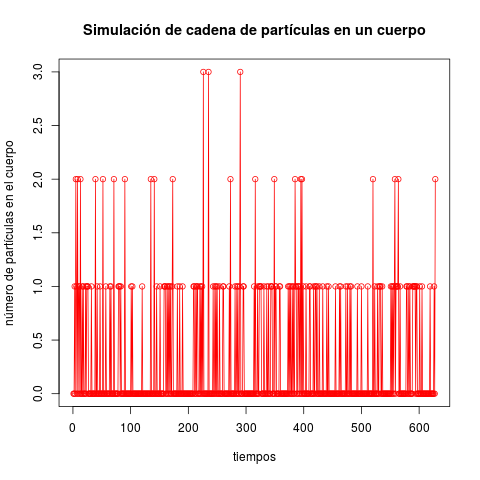
\includegraphics[scale=0.5]{ej3_1.png}
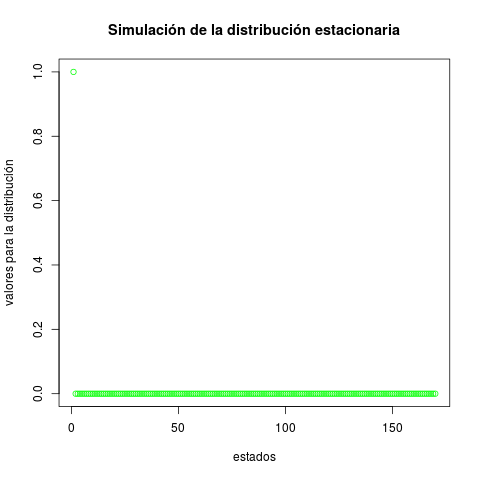
\includegraphics[scale=0.5]{ej3_2.png} 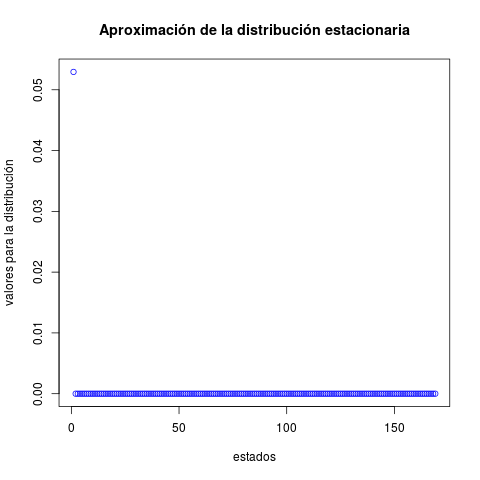
\includegraphics[scale=0.5]{ej3_3.png}
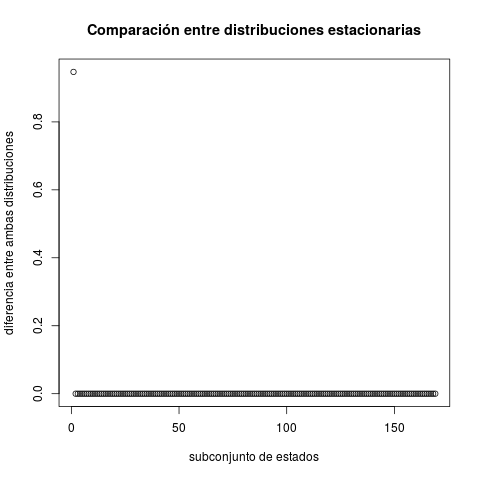
\includegraphics[scale=0.5]{ej3_4.png}

\section{Ejercicio 6}

\subsection{Código}

\lstinputlisting[language=R]{../ejercicio6.R}

\subsection{Gráficos}

\begin{center}
  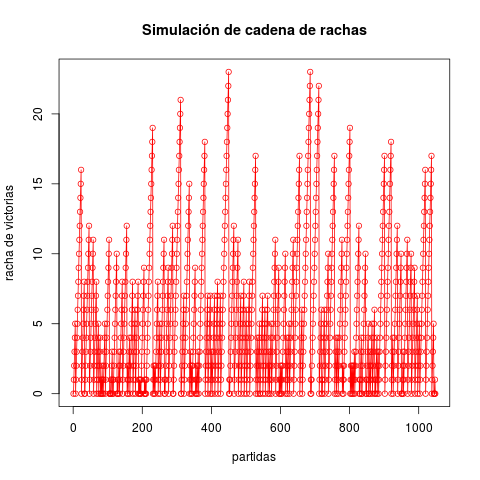
\includegraphics[scale=0.5]{ej6_1.png}
\end{center}
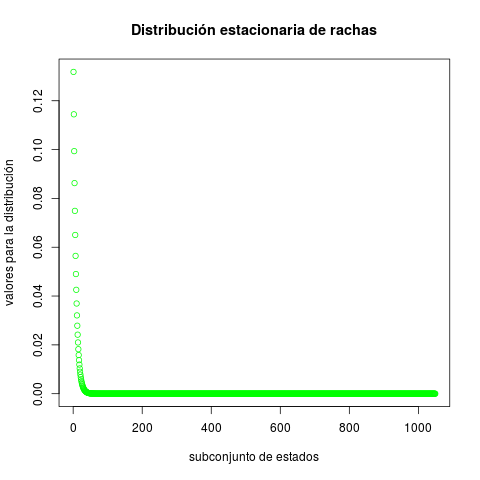
\includegraphics[scale=0.5]{ej6_2.png} 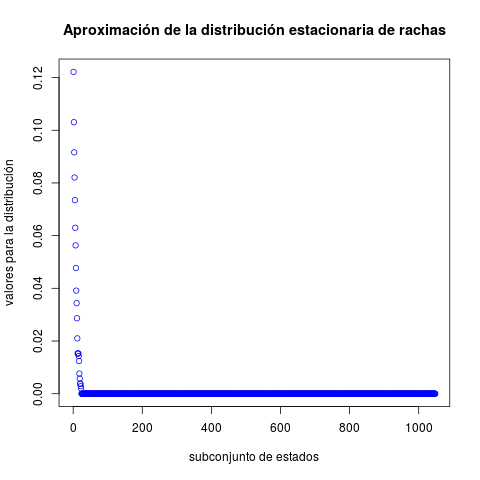
\includegraphics[scale=0.5]{ej6_3.png}
\begin{center}
  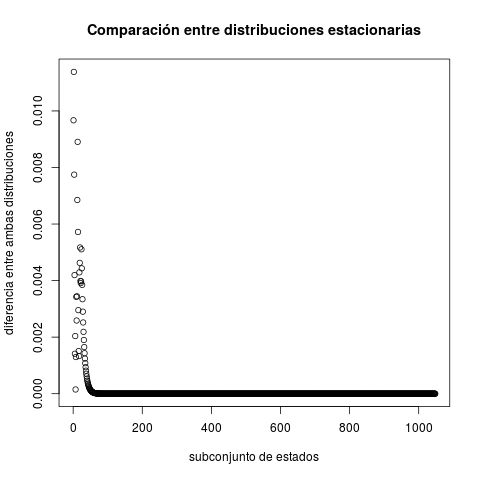
\includegraphics[scale=0.5]{ej6_4.png}
\end{center}

\newpage

\section{Ejercicio 7}

\subsection{Código}

\lstinputlisting[language=R]{../ejercicio7.R}
\par \par
Estimación de la esperanza de $T$ en una ejecución: $6{.}92568203198495$.

\subsection{Gráfico}

\begin{center}
  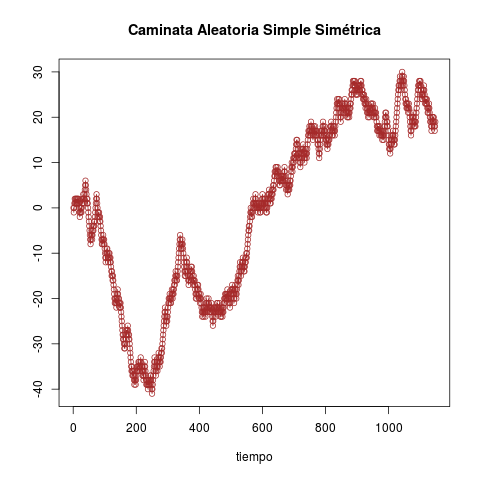
\includegraphics[scale=0.4]{ej7_1.png}
\end{center}

\section{Ejercicio 8}
\subsection{Código}
\lstinputlisting[language=R]{../ejercicio8.R}
\subsection{Gráficos}

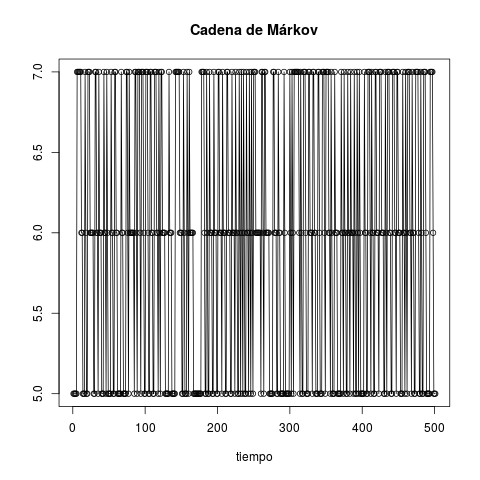
\includegraphics[scale=0.4]{ej8_1.png}
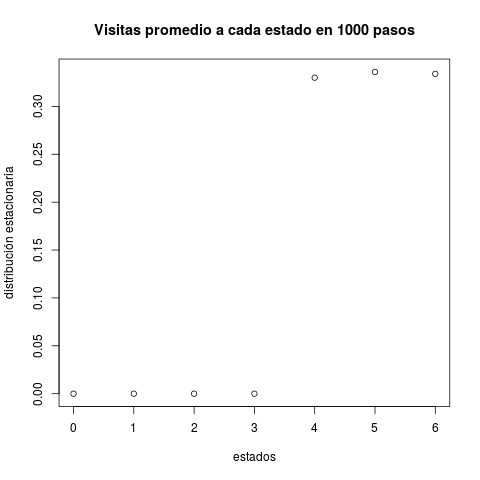
\includegraphics[scale=0.4]{ej8_2.png} \par
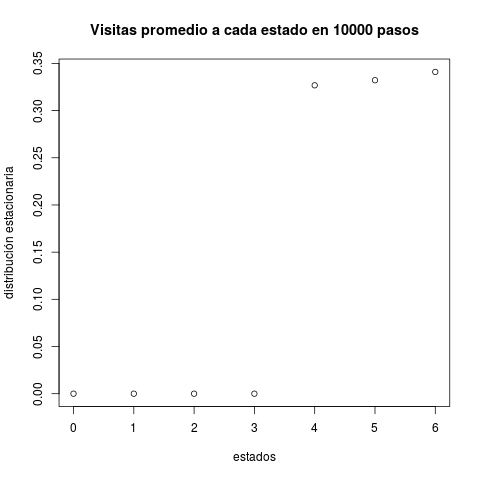
\includegraphics[scale=0.4]{ej8_3.png}
\newpage

\section{Ejercicio 11}

\subsection{Código}

Obsérvese que para la matriz de probabilidades de transición, los estados corresponden a:
\begin{itemize}
\item $0$ $=$ $CL$
\item $1$ $=$ $CN$
\item $2$ $=$ $NL$
\item $3$ $=$ $NN$.
\end{itemize}

\lstinputlisting[language=R]{../ejercicio11.R}

\subsection{Gráficos}

\begin{center}
  \makebox[\textwidth]{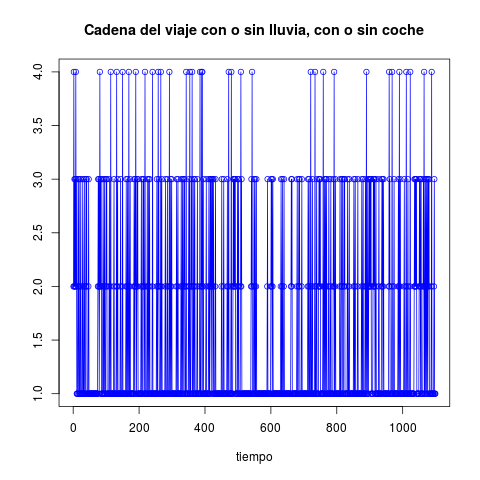
\includegraphics[scale=0.5]{ej11_1.png}}
\end{center}
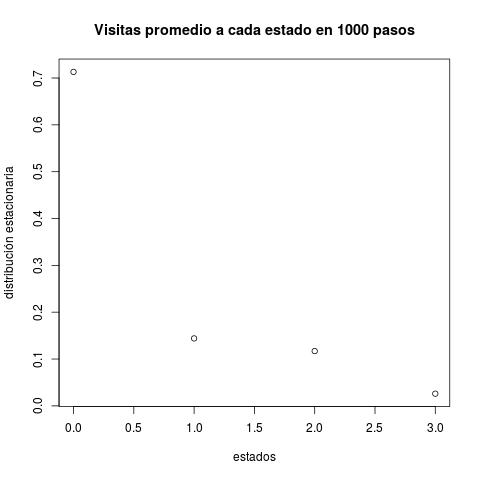
\includegraphics[scale=0.5]{ej11_2.png} 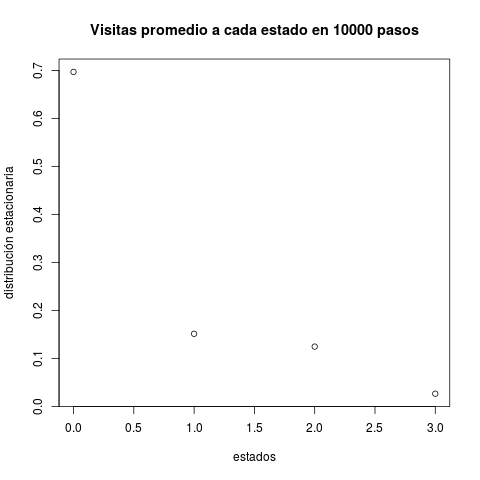
\includegraphics[scale=0.5]{ej11_3.png}

\end{document}
